\documentclass[floatsintext,man]{apa6}

\usepackage{amssymb,amsmath}
\usepackage{ifxetex,ifluatex}
\usepackage{fixltx2e} % provides \textsubscript
\ifnum 0\ifxetex 1\fi\ifluatex 1\fi=0 % if pdftex
  \usepackage[T1]{fontenc}
  \usepackage[utf8]{inputenc}
\else % if luatex or xelatex
  \ifxetex
    \usepackage{mathspec}
    \usepackage{xltxtra,xunicode}
  \else
    \usepackage{fontspec}
  \fi
  \defaultfontfeatures{Mapping=tex-text,Scale=MatchLowercase}
  \newcommand{\euro}{€}
\fi
% use upquote if available, for straight quotes in verbatim environments
\IfFileExists{upquote.sty}{\usepackage{upquote}}{}
% use microtype if available
\IfFileExists{microtype.sty}{\usepackage{microtype}}{}

% Table formatting
\usepackage{longtable, booktabs}
\usepackage{lscape}
% \usepackage[counterclockwise]{rotating}   % Landscape page setup for large tables
\usepackage{multirow}		% Table styling
\usepackage{tabularx}		% Control Column width
\usepackage[flushleft]{threeparttable}	% Allows for three part tables with a specified notes section
\usepackage{threeparttablex}            % Lets threeparttable work with longtable

% Create new environments so endfloat can handle them
% \newenvironment{ltable}
%   {\begin{landscape}\begin{center}\begin{threeparttable}}
%   {\end{threeparttable}\end{center}\end{landscape}}

\newenvironment{lltable}
  {\begin{landscape}\begin{center}\begin{ThreePartTable}}
  {\end{ThreePartTable}\end{center}\end{landscape}}




% The following enables adjusting longtable caption width to table width
% Solution found at http://golatex.de/longtable-mit-caption-so-breit-wie-die-tabelle-t15767.html
\makeatletter
\newcommand\LastLTentrywidth{1em}
\newlength\longtablewidth
\setlength{\longtablewidth}{1in}
\newcommand\getlongtablewidth{%
 \begingroup
  \ifcsname LT@\roman{LT@tables}\endcsname
  \global\longtablewidth=0pt
  \renewcommand\LT@entry[2]{\global\advance\longtablewidth by ##2\relax\gdef\LastLTentrywidth{##2}}%
  \@nameuse{LT@\roman{LT@tables}}%
  \fi
\endgroup}


  \usepackage{graphicx}
  \makeatletter
  \def\maxwidth{\ifdim\Gin@nat@width>\linewidth\linewidth\else\Gin@nat@width\fi}
  \def\maxheight{\ifdim\Gin@nat@height>\textheight\textheight\else\Gin@nat@height\fi}
  \makeatother
  % Scale images if necessary, so that they will not overflow the page
  % margins by default, and it is still possible to overwrite the defaults
  % using explicit options in \includegraphics[width, height, ...]{}
  \setkeys{Gin}{width=\maxwidth,height=\maxheight,keepaspectratio}
\ifxetex
  \usepackage[setpagesize=false, % page size defined by xetex
              unicode=false, % unicode breaks when used with xetex
              xetex]{hyperref}
\else
  \usepackage[unicode=true]{hyperref}
\fi
\hypersetup{breaklinks=true,
            pdfauthor={},
            pdftitle={Statistical Reanalysis of Munster Irish Stress: M3},
            colorlinks=true,
            citecolor=blue,
            urlcolor=blue,
            linkcolor=black,
            pdfborder={0 0 0}}
\urlstyle{same}  % don't use monospace font for urls

\setlength{\parindent}{0pt}
%\setlength{\parskip}{0pt plus 0pt minus 0pt}

\setlength{\emergencystretch}{3em}  % prevent overfull lines


% Manuscript styling
\captionsetup{font=singlespacing,justification=justified}
\usepackage{csquotes}
\usepackage{upgreek}



\usepackage{tikz} % Variable definition to generate author note

% fix for \tightlist problem in pandoc 1.14
\providecommand{\tightlist}{%
  \setlength{\itemsep}{0pt}\setlength{\parskip}{0pt}}

% Essential manuscript parts
  \title{Statistical Reanalysis of Munster Irish Stress: M3}

  \shorttitle{MI Stats}


  \author{Eileen Blum\textsuperscript{1}}

  % \def\affdep{{""}}%
  % \def\affcity{{""}}%

  \affiliation{
    \vspace{0.5cm}
          \textsuperscript{1} Rutgers University  }



  \abstract{This paper presents a new statistical analysis of Blum (2018)'s Munster
Irish (MI) acoustic data that uses linear mixed effects models. MI has
been described as presenting a stress pattern that current metrical and
non-metrical theories of stress, such as in Hayes (1995); deLacy (2002);
deLacy (2004); deLacy (2006), cannot account for: the ternary stress
attraction hierarchy of V \textless{} /ax/ \textless{} V\textipa{:}.
Blum (2018)'s acoustic study collected new data in order to reevaluate
evidence for the MI stress pattern. Blum (2018)'s statistical analysis
of the data from a single speaker of MI utilized t-tests to show that
previous work did not accurately decribe the stress pattern produced by
an MI speaker. Using linear mixed effects models provides a more
accurate measure of significance and variance while avoiding Type 1
errors (Winter, 2013) and this paper uses them to show that previous
descriptions may not have been so far off.}
  



  \usepackage{tipa}
  \usepackage{gb4e}
  \noautomath

\usepackage{amsthm}
\newtheorem{theorem}{Theorem}
\newtheorem{lemma}{Lemma}
\theoremstyle{definition}
\newtheorem{definition}{Definition}
\newtheorem{corollary}{Corollary}
\newtheorem{proposition}{Proposition}
\theoremstyle{definition}
\newtheorem{example}{Example}
\theoremstyle{definition}
\newtheorem{exercise}{Exercise}
\theoremstyle{remark}
\newtheorem*{remark}{Remark}
\newtheorem*{solution}{Solution}
\begin{document}

\maketitle

\setcounter{secnumdepth}{0}



\section{Introduction}\label{introduction}

The goal of this paper is to provide a statistical reanalysis of data
from a single native speaker of Munster Irish (MI) using linear mixed
effects models (Winter, 2013). Blum (2018)'s statistical analysis of the
speaker (M3)'s productions utilized t-tests to determine the
significance of the described stress pattern, syllable position, and
frame sentence for various acoustic properties. Using linear mixed
effects models provides a more accurate measure of significance and
variance while avoiding Type 1 errors.

Impressionistic descriptions of MI (Blankenhorn, 1981; Breatnach, 1947;
Gussman, 2002; Hickey, 2014; O'Rahilly, 1932; O'Siadhail, 1989; ÓCuív,
1944; Sé, 1989) agree that when a word consists of only short vowels
primary stress is on the first syllable. They also agree that if the
second syllable contains a long vowel, it will be stressed. In addition,
descriptions agree that the syllable {[}ax{]} can also attract stress,
as in {[}\textipa{b@"kax}{]}, but not away from a long vowel (i.e.
{[}\textipa{"}CV\textipa{:}.Cax{]}, *{[}CV\textipa{:"}Cax{]}); and that
coda consonants do not otherwise contribute to stress attraction. The MI
stress pattern has thus been described as having a three-way weight
distinction between short vowels, /ax/, and long vowels, as shown in
(\ref{ternaryweight}) below (Doherty 1991, Bennett 2015).

\begin{exe}
  \ex \label{ternaryweight}
  V < /ax/ < V\textipa{:}
\end{exe}

Blum (2018)'s statstical analysis found that stress did fall on the
second vowel in CVCax words and it was confirmed that the first vowel
reduces: i.e. /CVCax/ \(\rightarrow\) {[}C\textipa{@"}Cax{]}. However,
in all other word forms, it was argued that stress falls on the initial
syllable, even in words with the shape {[}CVCV\textipa{:}{]}. In
addition, it was argued that /a/ never reduces before {[}x{]}: i.e.
{[}\textipa{"}Cax.Cax{]}, *{[}Cax.C\textipa{@}x{]}. Evidence for stress
and resistance to vowel reduction was found in the first formant (F1).

The current paper will reevaluate M3's data using linear mixed effects
models. It will show that for two short vowels, {[}a{]} and
{[}\textipa{@}{]}, F1 varies based on an interaction between described
stress and syllable positions. The new analysis will find that when
these two vowels are stressed F1 is often higher, but the degree to
which they are distinguished from unstressed vowels differs based on
syllable position.

\section{Experimental Methods}\label{experimental-methods}

\subsection{Participant}\label{participant}

The single subject (M3) was a 74 year old male native speaker of Irish
from the Corca Dhuibhne Gaeltacht on the Dingle Peninsula. M3 spoke only
Irish until age 10, at which time he had a cleft palate repaired and
learned English during his hospital stay. M3 had a minor speech
impediment which made it difficult for him to produce coronal stops
({[}t{]}s were often fricated) and he has had limited contact with MI in
day-to-day life over the past 50 years. While his speech impediment does
not likely affect potential correlates of stress, it is possible that
the way he speaks is no longer the norm or understood by anyone outside
his family. Analyzing data from only one speaker has the possibility of
describing an idiolectal difference that is not representative of the
stress pattern produced more widely in MI, as it is used daily. However,
if the speaker is cognitively intact, his phonological system represents
a possible state of the Phonological Module, and so is relevant to
evaluating theories of that module's representational and computational
properties. I have reproduced the same experiment in multiple
gaeltachtaí of the Munster region of Ireland and in future work I plan
to analyze those field recordings for comparison and to determine the
stress correlates of MI across speakers and across counties in Munster.

\subsection{Stimuli}\label{stimuli}

The target words were existing MI words, initially collected from the
online pronunciation database at www.teanglann.ie (2013). The target
words were verified by two consulting native speakers of a Connacht
dialect and one native speaker of MI. The shapes of the target words
allowed comparison of the acoustic properties of {[}x{]}, {[}a{]},
{[}a\textipa{:}{]}, and other short and long vowels in both initial and
peninitial positions. I assumed that comparing properties of these
segments in different environments would be sufficient to identify
acoustic properties that differed significantly between these three
segments, and thus could be ascribed to phonological metrical
prominence.

MI stress has been described to fall mainly on the first or second
syllable of a word, so the target list was restricted to roots with two
syllables. Wug words were used when stimuli shapes were rare in the
www.teanglann.ie (2013) database. Vowel length and syllable shape were
controlled so as to test only the forms that are crucial to the
described stress pattern. The default stress pattern should be easily
detectable in words with two short vowels, as in (Table
\ref{stim_shape}a). In order to determine the acoustic properties that
differentiate stress on long and short vowels in MI, roots with a long
vowel in each position of a disyllabic word were also included, as in
(Table \ref{stim_shape}b). Lastly, the properties of the {[}ax{]}
syllable were tested in each position adjacent to a short and a long
vowel, as in (Table \ref{stim_shape}c). The word shapes in (Table
\ref{stim_shape}) are also marked with the expected position of stress,
based on traditional descriptions.

\begin{table}
  \caption{Stimuli Shapes}
  \begin{tabular}{c c c}
  (a) \textipa{"}CV.CV & (b) \textipa{"}CV\textipa{:}.CV        & (c)CV.\textipa{"}Cax\\
                       &    CV.\textipa{"}CV\textipa{:}           & \textipa{"}Cax.CV\\
                       & \textipa{"}CV\textipa{:}.CV\textipa{:} &   \textipa{"}CV\textipa{:}.Cax\\
                                     &                                        & Cax.\textipa{"}CV\textipa{:}\\  
                       &                                        & \textipa{"}Cax.Cax
  \label{stim_shape}
  \end{tabular}
\end{table}

The vowel and consonant qualities in each position were restricted to
include the vowels {[}i{]} and {[}u{]} (the most common vowels) and
crucially {[}a{]}, which occurs in the {[}ax{]} sequence. Some shapes
were rare, so a few words with {[}o{]} were also included. Vowel
identity was included as a factor in the statistical analysis since the
vowels vary in inherent duration and inherent F0.

While long vowels are reported to attract stress in MI, coda consonants
are not claimed to contribute to syllable weight. For this reason and to
restrict the number of shapes tested, no syllables with coda consonants
were included, except for the {[}Cax{]} syllables in
(\ref{stim_shape}c). Consonant voicing and manner can affect a preceding
vowel's length (vanSanten, 1992), so medial consonants were limited to
the voiceless stops ({[}p{]}, {[}t{]}, and {[}k{]}) and fricatives
({[}f{]}, {[}s{]}, and {[}x{]}). Voiceless intervocalic obstruents are
both easy to segment and have a smaller effect on preceding vowel
duration than do voiced obstruents (vanSanten (1992); p.528-9 and others
cited therein). Words with medial fricatives were also included in order
to increase the number of real-word stimuli.

There were a total of 69 target words. Seven words of each shape were
included, except for CV.Cax words -- 13 words were included because this
shape is crucial to the issue under contention. The target word list was
copied three times and randomized (using Microsoft Excel's RAND
function) to create three sets of stimuli, each with different orders.
The three sets of words were combined into a single list. Filler
sentences were inserted after every five stimuli.

\subsection{Procedure}\label{procedure}

PsychoPy2 (Pierce, 2009, 2015) was used to generate a presentation of
the stimuli such that each target word appeared alone on a computer
screen. The subject produced each target word within the two frame
sentences in (Table \ref{frames}). The subject saw the sentences and
practiced using them with a few words before the experiment began.
Target words were produced phrase-medially in order to avoid
phrase-final lengthening effects (vanSanten, 1992). Two sentences were
used to vary any prosodic (intensity) effects of focus on new vs.~old
information, following Shih (2016). M3 was recorded in his home and was
given the frame sentences to learn. He then began recording with
non-target words in order to familiarize himself with the task. He read
individual target words written in standard Irish orthography on a
computer screen. He then said the word out loud within each of the two
frame sentences, and pressed the space bar in order to move on to the
next word, continuing at his own pace.

\begin{table}
  \caption{Frame Sentences}
  \begin{tabular}{c c c c c c c c c}
  Frame 1:  & Dúirt                            & Bríd                     & an  & focal         & X & sular           & imigh                         & sí\\
            & du\textipa{:\*r\super ht\super j}.& \textipa{b\*ri:d\super j}.& an.  & \textipa{f2.kl}.& X & \textipa{s2.l\*r}.& \textipa{I.mIg}. & \textipa{Si:}\\
            & "Brid                            & said the word X before leaving"\\
  Frame 2:  & Abair            & X  & faoi                & d'anáil\\
            & \textipa{a.b\*r}.& X  & \textipa{fsuper wi}.& d'a.nal\textipa{\super j}\\
            & "Say             & X under your breath"\\
  \label{frames}
  \end{tabular}
\end{table}

Recordings were made using a head-mounted AKG C420 condenser microphone
in order to maintain a constant distance between the mouth and the
microphone, with the goal of eliminating amplitude variation due to head
movement. The microphone was connected to a Marantz PMD670 solid state
recorder, which recorded using 44.1 kHz sample rate and 16 bit
quantization rate in mono. The data was saved as a RIFF (.wav) file to
ensure that no information was lost due to a lossy compression codec.
The participant's recordings were saved in a coded file, which was then
segmented manually using Praat (Boersma \& Weenink, 2013).

Segmentation was done by hand using primarily the waveform and
secondarily F2 to determine where segments began and ended. Vowels were
taken to begin at the zero-crossing of the first upswing of the first
non-deformed period and ended at the zero-crossing of the last downswing
of the last non-deformed period. If the boundary was unclear based on
the waveform, vowel boundaries were determined by the presence of a
robust F2 in the spectrogram, as long as there was a robust F1
underneath. Fricatives were taken to begin at the zero-crossing of the
first downswing of the last non-deformed period of the preceding vowel
and ended at the zero-crossing of the first upswing of the first
non-deformed period of the following vowel. Fricatives boundaries were
confirmed by the onset and offset of noise in the spectrogram.

\section{Statistical Analysis}\label{statistical-analysis}

\subsection{Previous Findings}\label{previous-findings}

Blum (2018)'s statistical analysis utilized Student's t-tests in
Microsoft Excel to determine where there was variation within the M3
data. The t-tests were used to determine which acoustic properties
correlate with word-level stress. The previous analysis assumed a
restricted p-value threshold of 0.01 rather than the more generous
standard of 0.05 in order to adjust for family-wise error and avoid
capitalizing on chance, but the possibility of committing a Type 1 error
remained due to the high number of tests run on the single dataset.

Blum (2018)'s t-test analysis found that stress did fall on the second
vowel, but only in CVCax words and it was confirmed that the first vowel
reduces: i.e. /CVCax/ \(\rightarrow\) {[}C\textipa{@"}Cax{]}. In all
other word forms, it was argued that stress falls on the initial
syllable, even in words with the shape {[}CVCV\textipa{:}{]}. In
addition, it was argued that /a/ never reduces before {[}x{]}: i.e.
{[}\textipa{"}Cax.Cax{]}, *{[}Cax.C\textipa{@}x{]}. Evidence for stress
and resistance to vowel reduction was found in the first formant (F1).
The vowels {[}a{]} and {[}\textipa{@}{]} were found to significantly
differ in height, but their distribution was not indicative of the
traditionally described stress pattern. For example, an initial short
{[}a{]} adjacent to a long vowel did not reduce, but adjacent to an
{[}ax{]} syllable it did. Crucially, F1 was also claimed to indicate
that the vowel in an {[}ax{]} syllable does not reduce to generate
{[}\textipa{@}x{]}.

\subsection{Reanalysis Methods}\label{reanalysis-methods}

The current analysis of M3's data uses linear mixed effects models in R
(R Core Team, 2016) via the lmer function of the lme4 package (Bates,
Mächler, Bolker, \& Walker, 2015). Separate models were built for each
of two vowels ({[}a{]} and {[}\textipa{@}{]}) and each of three acoustic
properties (vowel duration, F1, and F2). Data was organized in long
format such that each variable occupied a separate column and each row
contained a single vowel's data. Rows were labeled with the word,
syllable shape, and vowel (as it was segmented) in separate columns in
that order. To the right of the vowel label were the continuous
variables duration, F1, F2, F3 in order. Each vowel was also coded for
the categorical variables frame sentence (1 or 2), syllable position (1
or 2), and stress (0 or 1 according to the descriptions).

\section{Results}\label{results}

The lmer() function was used to separately model each of the continous
dependent variables (duration, F1, and F2) as a function of the three
fixed effects (frame, syllable, and stress). In addition, the mixed
effects models encoded a random effect of word, which was labeled by the
file name. Statistical significance was assessed using hierarchical
partitioning of variance via nested model comparisons. Models were
compared using the anova() function. Visual inspection of residual plots
revealed both normal distribution and homoskedasticity.

\subsection{Short {[}a{]} vowels}\label{short-a-vowels}

Short {[}a{]} vowels include all vowels marked as {[}a{]} during
segmentation. These include both those in /ax/ syllables and those that
are not. Whether or not they were marked as stressed (1), depends upon
the other vowel present in the word. So {[}a{]} vowels, whether or not
they are in an /ax/ syllable, would be marked as unstressed (0) if the
other vowel in the word is long, for example.

\subsubsection{Duration}\label{duration}

Stress and syllable position were shown to have a significant effect on
the duration of {[}a{]} vowels (p \textless{} 0.05), but frame sentence
did not. There was a main effect of stress on duration
(\textipa{X}\textsuperscript{2}(1)=0.97, p=3.255e-01) and syllable
position on duration (\textipa{X}\textsuperscript{2}(1)=26.443,
p=2.714e-07). No effect of frame sentence was found. The interaction
between stress and syllable position was found not to have a significant
effect on duration (\textipa{X}\textsuperscript{2}(1)=3.4548,
p=0.06307).

\subsubsection{F1}\label{f1}

Stress was shown to have a significant effect on the F1 of {[}a{]}
vowels, but neither syllable position nor frame sentence did. There was
a main effect of stress on F1 (\textipa{X}\textsuperscript{2}(1)=27.966,
p=1.235e-07). The effect of syllable position on F1 was shown not to be
significant (\textipa{X}\textsuperscript{2}(1)=0.2704, p=0.6031). No
effect of frame sentence was found. The interaction between stress and
syllable positions was found to significantly effect F1
(\textipa{X}\textsuperscript{2}=14.977, p=0.0001088).

\subsubsection{F2}\label{f2}

No categorical factors were shown to have a significant effect on F2.
The effects of both stress (\textipa{X}\textsuperscript{2}(1)=1.337,
p=0.25) and syllable position (\textipa{X}\textsuperscript{2}(1)=2.89,
p=0.089) were found not to be significant. No effect of frame sentence
was found. The interaction between stress and syllable position was
found not to significantly affect F2
(\textipa{X}\textsuperscript{2}=0.0061, p=0.93756).

\subsection{\texorpdfstring{{[}\textipa{@}{]}
Vowels}{{[}{]} Vowels}}\label{vowels}

{[}\textipa{@}{]} vowels include all vowels marked as {[}\textipa{@}{]}
during segmentation. These include both {[}\textipa{@}{]} in /ax/
syllables and those that are not. There are stressed {[}\textipa{@}{]}
vowels in the two C\textipa{@}C\textipa{@} words, which were also
extremely common words---{[}\textipa{"p@t@}{]} \enquote{(cooking) pot}
and {[}\textipa{"k@p@}{]} \enquote{(drinking) cup}. According to Green
(1996:4) it is possible that the schwas in stressed syllables are
underlying and not the result of vowel reduction.

\subsubsection{Duration}\label{duration-1}

All three categorical predictors were shown to have a significant effect
on \textipa{@} duration. There was a main effect of stress
(\textipa{X}\textsuperscript{2}(1)=29.827, p=4.723e-08), syllable
position (\textipa{X}\textsuperscript{2}(1)=48.692, p=2.996e-12), and
frame sentence (\textipa{X}\textsuperscript{2}(1)=15.954, p=6.489e-05).
The interaction between stress and syllable position was found to
significantly affect {[}\textipa{@}{]} duration
(\textipa{X}\textsuperscript{2}=17.022, p=3.695e-05).

\subsubsection{F1}\label{f1-1}

All three categorical predictors were also shown to have a significant
effect on the F1 of \textipa{@}. There was a main effect of stress
(\textipa{X}\textsuperscript{2}(1)=9.5367, p=0.002014), syllable
position (\textipa{X}\textsuperscript{2}(1)=6.4637, p=0.01101), and
frame sentence (\textipa{X}\textsuperscript{2}(1)=40.431, p=2.036e-10).
The interaction between stress and syllable position was shown to
significantly affect F1 of \textipa{@}
(\textipa{X}\textsuperscript{2}=10.6015, p=0.00113).

\subsubsection{F2}\label{f2-1}

Only frame sentence significantly affected the F2 of \textipa{@} vowels.
The effect of stress (\textipa{X}\textsuperscript{2}(1)=0.4965, p=0.481)
and syllable position (\textipa{X}\textsuperscript{2}(1)=0.0069,
p=0.9338) on F2 were shown not to be significant. There was, however, a
main effect of frame sentence (\textipa{X}\textsuperscript{2}(1)=22.432,
p=2.177e-06). The interaction between stress and syllable position was
found not to have a significant effect on \textipa{@} F2
(\textipa{X}\textsuperscript{2}=0.9324, p=0.3342).

\subsection{Summary}\label{summary}

The described stress pattern was shown to be a significant predictor of
duration and F1 for both short {[}a{]} and {[}\textipa{@}{]} vowels.
Duration of {[}a{]} as well as duration and F1 of {[}\textipa{@}{]} were
predicted by syllable position. F2 was not predicted by any of the
categorical factors for {[}a{]}, but was predicted by frame sentence for
{[}\textipa{@}{]} vowels. The interaction between stress and syllable
position was shown to be a significant predictor of F1 for {[}a{]} as
well as duration and F1 for {[}\textipa{@}{]} vowels.

\section{Discussion}\label{discussion}

Blum (2018) claims that F1 is the only significant acoustic correlate of
stress such that stressed {[}a{]} vowels are more peripheral and
unstressed {[}a{]} vowels are reduced to {[}\textipa{@}{]}. Blum (2018)
further claims that F1 only varies based on syllable position so
stressed vowels are always initial, except in CVCax words and this is
due to some pressure against reducing an {[}a{]} vowel before {[}x{]}.
Blum (2018)'s analysis thus suggests that traditional descriptions may
have been right about CVCax words, but otherwise the acoustic measures
showed more variation based on syllable position.

The linear mixed effects model analysis in this paper shows that
particularly F1 of both {[}a{]} and {[}\textipa{@}{]} vowels was
significantly affected by an interaction between the described stress
pattern and syllable position. Figure 1 demonstrates the interaction
between stress and syllable position because while durations don't
necessarily differ by stress, the distribution of stressed
{[}\textipa{@}{]} durations (the blue boxes) is constrained by syllable
position. So, in the first syllable there are more stressed
{[}\textipa{@}{]} that have a longer average duration than unstressed
{[}\textipa{@}{]}, but in the second syllable there are more unstressed
{[}\textipa{@}{]} vowels that have a longer average duration. A similar
distribution can be seen for {[}a{]} durations in Figure 2, which shows
that there are stressed {[}a{]} in an initial syllable which are shorter
than any unstressed {[}a{]}.

\begin{figure}
\centering
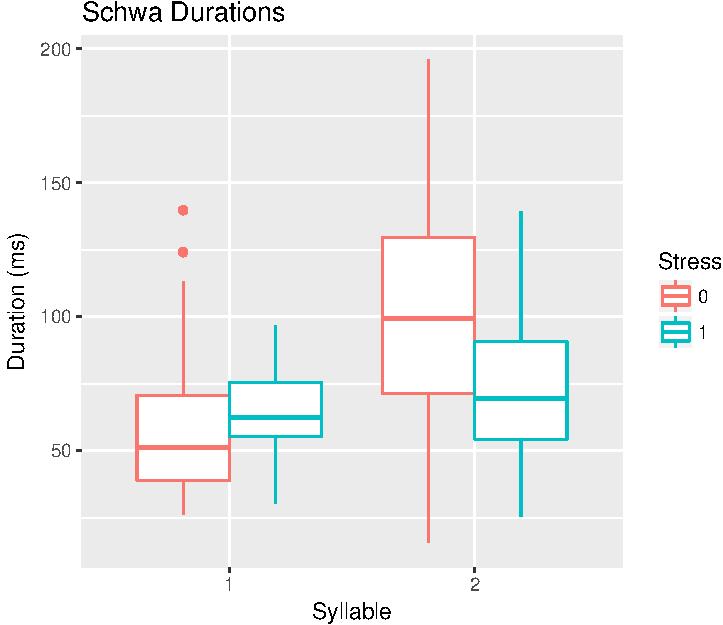
\includegraphics{mistress_restat_files/figure-latex/durplot-1.pdf}
\caption{}
\end{figure}

A similar distribution can be seen for {[}a{]} durations in Figure 2,
which shows that there are stressed {[}a{]} in an initial syllable which
are shorter than any unstressed {[}a{]}.

\begin{figure}
\centering
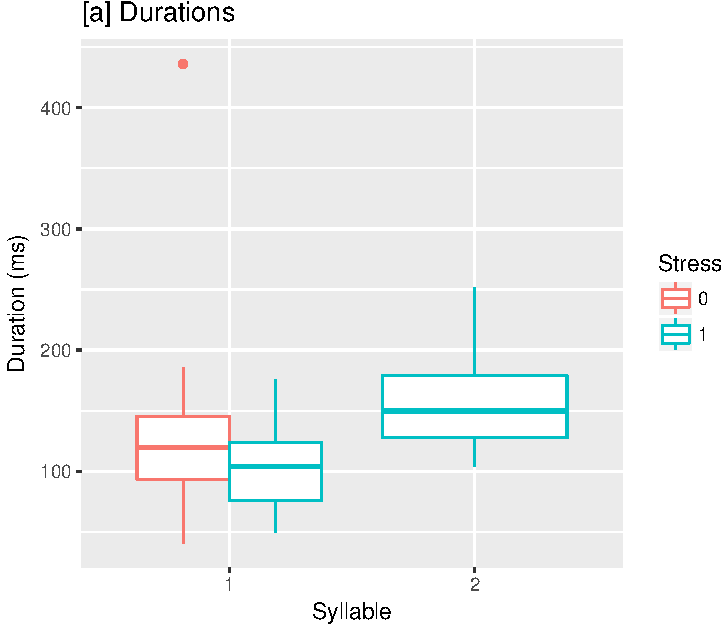
\includegraphics{mistress_restat_files/figure-latex/adurplot-1.pdf}
\caption{}
\end{figure}

F1, on the other hand, show a distribution more like what one might
expect for the perceptual saliency of stressed vs.~unstressed vowels.
There is much less overlap in the F1 values of stressed and unstressed
vowels and the stressed vowels have higher F1, which means they are
lower (i.e.~more peripheral) than unstressed vowels. For example, Figure
3 shows that F1 of stressed {[}\textipa{@}{]} was higher on average than
unstressed {[}\textipa{@}{]}. While this generalization holds in both
syllable positions the difference between stressed and unstressed
{[}\textipa{@}{]} is more pronounced in initial syllables.

\begin{figure}
\centering
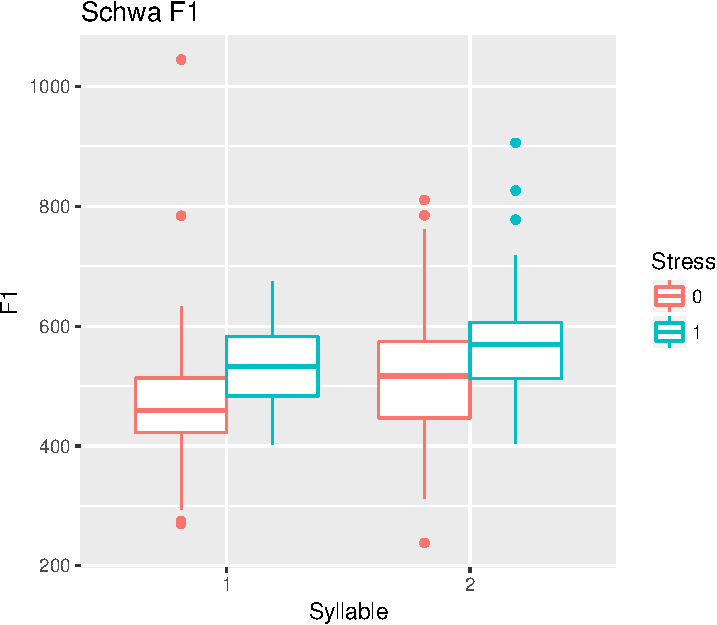
\includegraphics{mistress_restat_files/figure-latex/f1plot-1.pdf}
\caption{}
\end{figure}

Figure 4 shows the same pattern for F1 values of {[}a{]}, which are
noticably higher for stressed than unstressed vowels in initial
syllables.

\begin{figure}
\centering
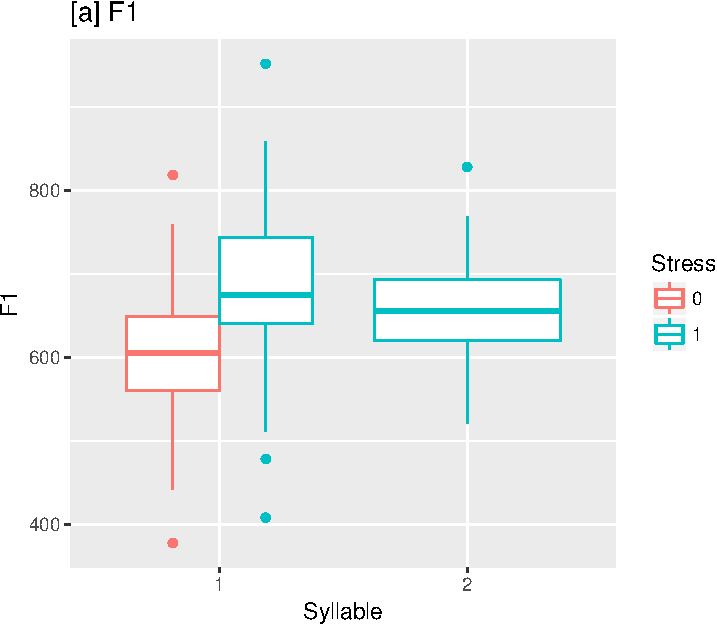
\includegraphics{mistress_restat_files/figure-latex/af1plot-1.pdf}
\caption{}
\end{figure}

F2 was only affected by frame sentence, which does not provide
information relevant to determining M3's stress pattern.

\section{Conclusion}\label{conclusion}

This paper provides a new statistical analysis of Blum (2018)'s acoustic
production data from a single speaker of Munster Irish. Blum (2018)
utilized Student's t-tests to show that vowel reduction indicated by F1
demontrated a stress pattern that differs from the pattern that has been
described. This paper uses linear mixed effects models to show that for
two short vowels, {[}a{]} and {[}\textipa{@}{]}, an interaction between
the described stress pattern and syllable position constrains the
distribution of F1 values such that stressed {[}a{]} and
{[}\textipa{@}{]} are lower when stressed. In addition, stress affected
vowel duration, but whether stressed vowels were longer or shortered
differed depending upon the syllable position. In short, the stress
pattern described by previous impressionistic work may not be as
inaccurate as Blum (2018) suggests.

Further work remains to determine M3's complete stress pattern. The next
steps for this analysis will be to determine the effect of stress,
syllable position, and frame sentence on high vowels. In addition,
future work will include analysis of long vowels and independently
testing short vowels and /ax/ vowels in order to determine if there is
any difference in the effects of stress and syllable position on those
two type of vowels.

\newpage

\section{References}\label{references}

\setlength{\parindent}{-0.5in} \setlength{\leftskip}{0.5in}

\hypertarget{refs}{}
\hypertarget{ref-R-lme4}{}
Bates, D., Mächler, M., Bolker, B., \& Walker, S. (2015). Fitting linear
mixed-effects models using lme4. \emph{Journal of Statistical Software},
\emph{67}(1), 1--48.
doi:\href{https://doi.org/10.18637/jss.v067.i01}{10.18637/jss.v067.i01}

\hypertarget{ref-blankenhorn1981}{}
Blankenhorn, V. (1981). Pitch, quantity and stress in munster irish.
\emph{Éigse}, \emph{18}(2), 225--250.

\hypertarget{ref-blum2018}{}
Blum, E. (2018, January). \emph{Allophony-driven stress in munster
irish}. Rutgers University.

\hypertarget{ref-praat}{}
Boersma, P., \& Weenink, D. (2013). \emph{Praat: Doing phonetics by
computer}. Retrieved from \url{http://www.praat.org/}

\hypertarget{ref-breatnach1947}{}
Breatnach, R. (1947). \emph{The irish of ring, co. waterford}. Dublin
Institute for Advanced Studies.

\hypertarget{ref-delacy2002}{}
deLacy, P. (2002). \emph{The formal expression of markedness}
(PhD thesis). University of Massachusetts Amherst.

\hypertarget{ref-delacy2004}{}
deLacy, P. (2004). Markedness conflation in optimality theory.
\emph{Phonology}, \emph{21}.

\hypertarget{ref-delacy2006}{}
deLacy, P. (2006). Markedness: Reduction and preservation in phonology.
\emph{Cambridge Studies in Linguistics},
\emph{112}(doi:10.1017/CBO9780511486388).

\hypertarget{ref-gussman2002}{}
Gussman, E. (2002). Phonology: Analysis and theory. In. Cambridge
University.

\hypertarget{ref-hayes95}{}
Hayes, B. (1995). \emph{Metrical stress theory}. University of Chicago
Press.

\hypertarget{ref-hickey2014}{}
Hickey, R. (2014). The sound structure of irish. In \emph{Empirical
approaches to language typology} (Vol. 47). De Gruyter Mouton.

\hypertarget{ref-orahilly1932}{}
O'Rahilly, T. (1932). \emph{Irish dialects past and present: With
chapters on scottish and manx}. Dublin institute for advanced studies.

\hypertarget{ref-osiadhail1989}{}
O'Siadhail, M. (1989). \emph{Modern irish: Grammatical structure and
dialectal variation}. Cambridge University Press.

\hypertarget{ref-ocuiv1944}{}
ÓCuív, B. (1944). \emph{The irish of west muskerry, co. cork}. Dublin
Institute for Advanced Studies.

\hypertarget{ref-psychopy2}{}
Pierce, J. (2009). Generating stimuli for neuroscience using psychopy.
\emph{Frontiers in Neuroinformatics}, \emph{2}.

\hypertarget{ref-psychopy}{}
Pierce, J. (2015). \emph{PsychoPy: For stimulus generation and
experimental control in python}. Retrieved from
\url{http://www.psychopy.org}

\hypertarget{ref-R-base}{}
R Core Team. (2016). \emph{R: A language and environment for statistical
computing}. Vienna, Austria: R Foundation for Statistical Computing.
Retrieved from \url{https://www.R-project.org/}

\hypertarget{ref-ose1989}{}
Sé, D. Ó. (1989). Contributions to the study of word stress in irish.
\emph{Ériu}, \emph{40}.

\hypertarget{ref-shih2016}{}
Shih, S.-h. (2016). \emph{On the existence of sonority-driven stress in
gujarati}.

\hypertarget{ref-vanSanten92}{}
vanSanten, J. (1992). Contextual effects on vowel duration. \emph{Speech
Communication}, \emph{11}.

\hypertarget{ref-Winter-lmer}{}
Winter, B. (2013). \emph{Linear models and linear mixed effects models
in r with linguistic applications}. Retrieved from
\url{http://arxiv.org/pdf/1308.5499.pdf}






\end{document}
